实验的搭建和实施主要借助 MATLAB 与 Simulink 完成。

\begin{figure}[htbp]
    \centering
    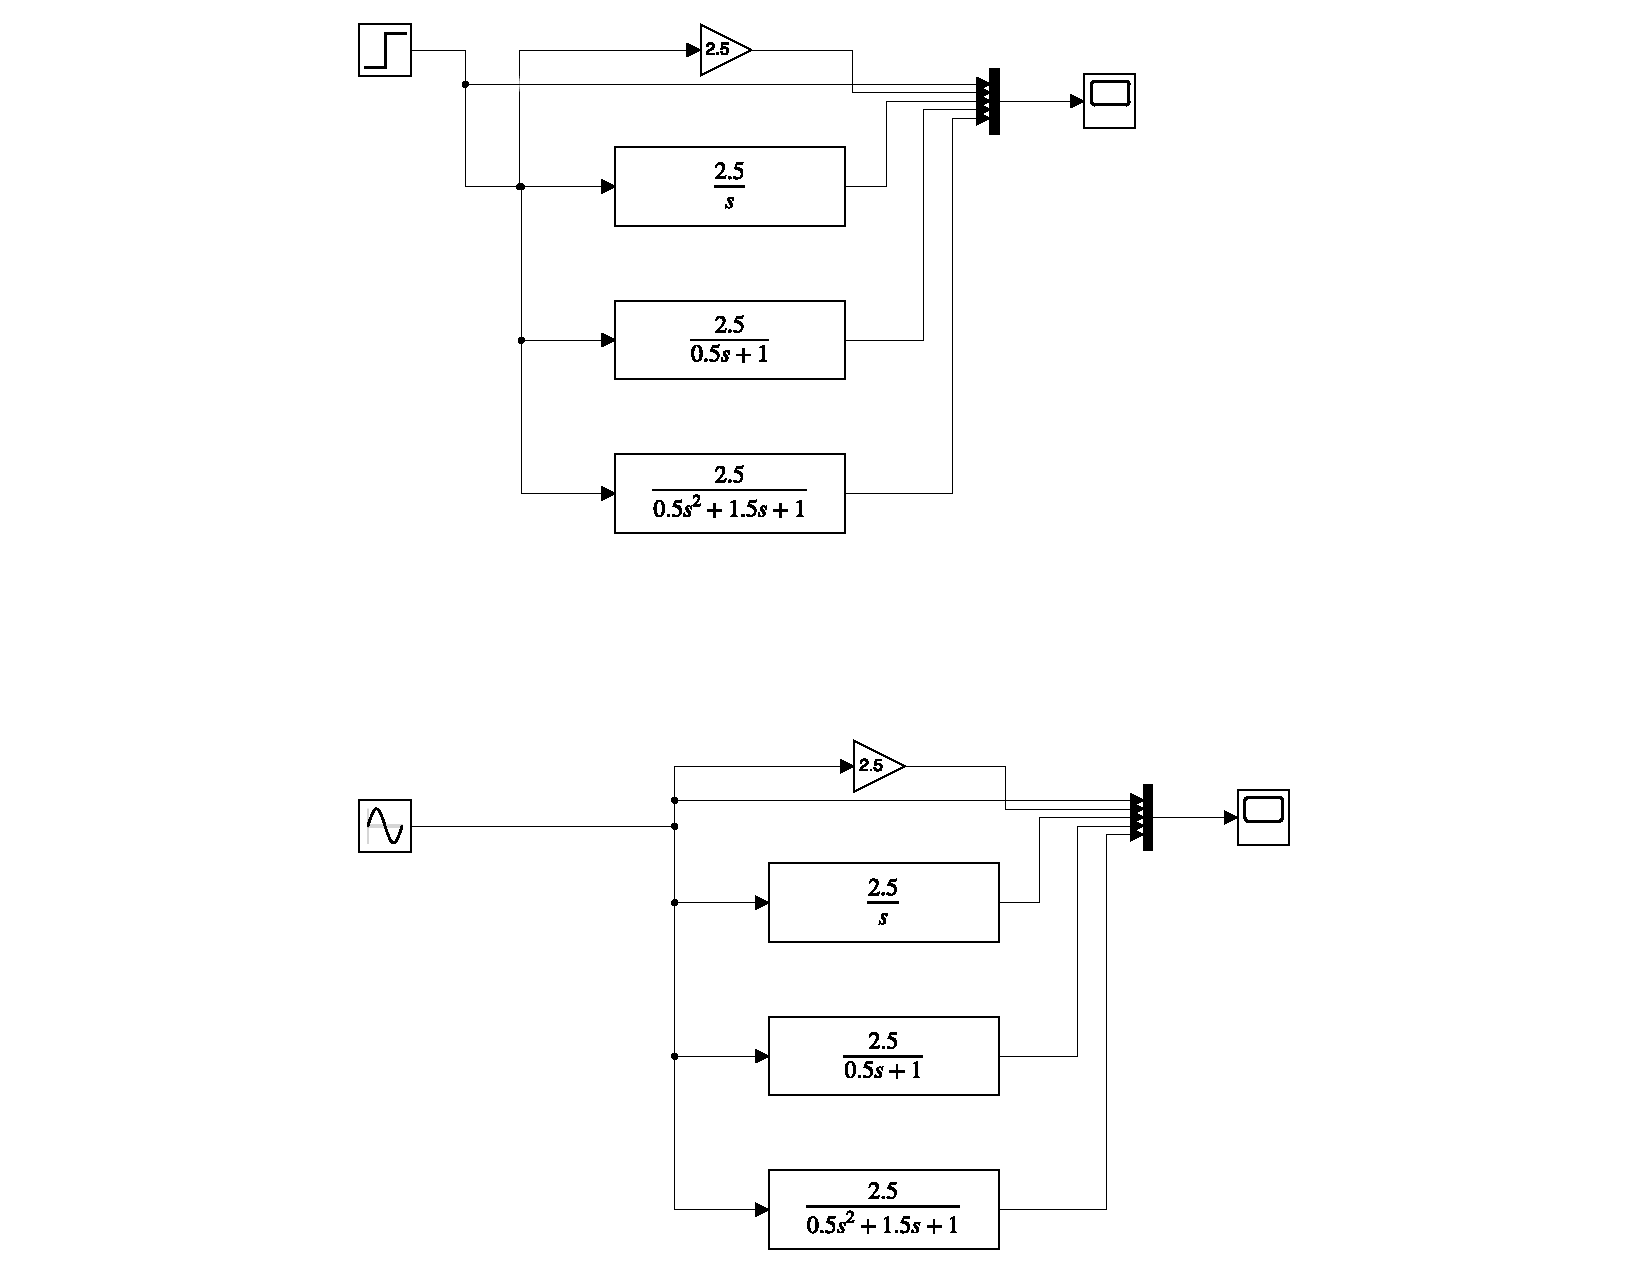
\includegraphics[width=0.8\linewidth]{../figures/V1.pdf}
    \caption{Simulink 模型}
\end{figure}

在 Simulink 模型中实现具有给定参数的传递环节（P、I、PT1 和 PT2 环节），例如 $K_P = 2$、$T_1 = \SI{0.5}{\second}$ 和 $T_2 = \SI{0.5}{\second}$，以生成其阶跃响应。
